\documentclass[11pt]{article}
\usepackage[margin=18mm,headheight=22pt]{geometry}
\usepackage{amsmath}
\usepackage{fontspec}
\usepackage{unicode-math}
\setmainfont{NewCM10}[Extension=.otf,UprightFont=*-Book,BoldFont=*-Bold,ItalicFont=*-BookItalic,BoldItalicFont=*-BoldItalic]
\setsansfont{NewCMSans10}[Extension=.otf,UprightFont=*-Book,BoldFont=*-Bold,ItalicFont=*-BookOblique,BoldItalicFont=*-BoldOblique]
\setmathfont{NewCMMath-Book.otf}
\usepackage{xcolor}
\definecolor{FAUblue}{HTML}{04316A}
\definecolor{Paperblue}{HTML}{EEF2F7}
\definecolor{EEIgold}{HTML}{CC9C42}
\usepackage{etoolbox,enumitem,booktabs,tabularx,array,needspace,microtype}
\usepackage[most]{tcolorbox}
\usepackage{titlesec,fancyhdr}
\usepackage[hidelinks]{hyperref}
\usepackage{draftwatermark}
\SetWatermarkText{Made by Thanate Amornjiraporn (Focus)}
\SetWatermarkColor{black!7}\SetWatermarkFontSize{30pt}\SetWatermarkAngle{45}
\setlength{\parindent}{0pt}
\setlength{\parskip}{5pt}
\setlist{itemsep=2pt,topsep=3pt,leftmargin=1.6em,beginpenalty=10000,endpenalty=10000}
\raggedbottom
\clubpenalty=10000 \widowpenalty=10000 \displaywidowpenalty=10000 \interlinepenalty=10000
\setcounter{secnumdepth}{0}
\setcounter{tocdepth}{1}
\pagestyle{fancy}\fancyhf{}
\fancyhead[L]{\small\sffamily\color{FAUblue} From Fundamentals to AI Apocalypse · APDR · Chapter 11}
\fancyhead[R]{\small\sffamily Classes and Inheritance}
\fancyfoot[C]{\small\thepage}
\titleformat{\section}{\Large\bfseries\sffamily\color{FAUblue}}{}{0pt}{}
\titleformat{\subsection}{\large\bfseries\sffamily\color{FAUblue}}{}{0pt}{}
\titlespacing*{\section}{0pt}{16pt}{6pt}
\preto\section{\Needspace{8\baselineskip}}
\preto\subsection{\Needspace{6\baselineskip}}
\newtcolorbox{equationcard}[1]{colback=Paperblue,colframe=Paperblue,boxrule=0pt,arc=0pt,left=10pt,right=10pt,top=6pt,bottom=6pt,title={#1},fonttitle=\small\bfseries\sffamily,coltitle=FAUblue,before skip=8pt,after skip=8pt}
\newtcolorbox{workedbox}[1]{colback=white,colframe=EEIgold,boxrule=0pt,leftrule=3pt,arc=0pt,left=10pt,top=4pt,bottom=4pt,title={#1},fonttitle=\small\bfseries\sffamily,coltitle=FAUblue,attach title to upper={\par},before skip=8pt,after skip=8pt}
\newtcolorbox{recallbox}[1]{colback=white,colframe=FAUblue,boxrule=0pt,leftrule=3pt,arc=0pt,left=10pt,top=4pt,bottom=4pt,title={#1},fonttitle=\small\bfseries\sffamily,coltitle=FAUblue,attach title to upper={\par},before skip=8pt,after skip=8pt}
\usepackage{environ}
\newsavebox\measurebox
% Typeset the section once invisibly to measure it; start a new page if it will not fit in what is left.
\makeatletter
\newif\ifkeep@measuring
\NewEnviron{keepsection}{%
  \ifkeep@measuring \BODY \else
    \edef\keep@sec{\the\value{section}}\edef\keep@sub{\the\value{subsection}}%
    \setbox\measurebox\vbox{\hsize\linewidth\keep@measuringtrue\def\Needspace##1{}\BODY}%
    \setcounter{section}{\keep@sec}\setcounter{subsection}{\keep@sub}%
    \dimen2=\ht\measurebox \advance\dimen2\dp\measurebox
    \dimen@=\textheight
    \ifdim\pagegoal<\maxdimen
      \dimen@=\pagegoal \advance\dimen@-\pagetotal
      \ifdim\dimen2>\dimen@ \clearpage \dimen@=\textheight \fi
    \fi
    % if it fits, nothing inside may force an early break
    \ifdim\dimen2>\dimen@ \BODY \else \begingroup\def\Needspace##1{}\BODY\endgroup \fi
  \fi}
\makeatother
\newtcolorbox{notebox}{colback=Paperblue,colframe=Paperblue,boxrule=0pt,arc=0pt,left=8pt,right=8pt,top=4pt,bottom=4pt,before skip=6pt,after skip=6pt}
\newtcolorbox{plainbox}{colback=white,colframe=FAUblue,boxrule=0pt,leftrule=3pt,arc=0pt,left=10pt,right=8pt,top=4pt,bottom=4pt,before skip=6pt,after skip=8pt}
\usetikzlibrary{arrows.meta}
\title{\sffamily\bfseries\color{FAUblue}Classes and Inheritance}
\author{Algorithms, Programming, and Data Representation \ensuremath{\cdot} Module 92313 \ensuremath{\cdot} Chapter 11\\[2pt]\small From Fundamentals to AI Apocalypse · personal study guide}
\date{}
\begin{document}
\maketitle
\begingroup\footnotesize\setlength{\parskip}{0pt}\tableofcontents\endgroup
\clearpage

\Needspace{9\baselineskip}
{\large Keep an object’s data behind a stable interface, extend a class through inheritance, and trace which implementation Python finds first. Then use shared class state to give Rabbit objects IDs and meaningful operators.}


\begin{keepsection}
\Needspace{13\baselineskip}
\section{Start from memory}

\Needspace{10\baselineskip}
Answer before reading.

\Needspace{8\baselineskip}
\begin{enumerate}
\item Why call \texttt{get\_age()} instead of reading \texttt{age} directly?
\item Where does Python search for an inherited method?
\item What does a subclass do when it needs to initialise its own state and its parent’s?
\item How can a class variable provide unique IDs?
\item Why can comparing Rabbit parents with \texttt{==} recurse?
\end{enumerate}

\nopagebreak[4]{\small\itshape Answers: see “Start from memory” under Answers at the end.}
\end{keepsection}

\begin{keepsection}
\Needspace{16\baselineskip}
\section{How to use this guide}

\Needspace{13\baselineskip}
When tracing a call, write the instance type, the search order, and the first class that defines the method.

\Needspace{10\baselineskip}
\begin{enumerate}
\item \textbf{Day 0:} §11.1–11.3; practice 1, 2, 3, 11, 14.
\item \textbf{Day 1:} §11.4–11.5; practice 4, 5, 8, 9, 15, 16.
\item \textbf{Day 3:} §11.6–11.7; practice 6, 7, 10, 12, 13, 17, 18.
\item \textbf{About day 7:} Rebuild the inheritance and Rabbit derivations; solve 19–20.
\item \textbf{About day 14:} Work both exam problems without notes.
\item \textbf{Before the exam:} Tick only skills you can demonstrate from memory.
\end{enumerate}

\begin{notebox}\textbf{When stuck:} draw the class chain and mark the first definition Python finds.\end{notebox}
\end{keepsection}

\begin{keepsection}
\Needspace{16\baselineskip}
\section{How the chapter fits together}

\Needspace{13\baselineskip}
Accessors separate callers from representation. Inheritance reuses and extends behaviour; method lookup chooses the nearest definition. A class variable shares a counter, while special methods connect the class to Python operators.

\Needspace{6\baselineskip}
\textbf{Encapsulate}

\Needspace{4\baselineskip}
\begin{itemize}
\item \Needspace{4\baselineskip}
\textbf{Getter/setter} \hfill{\small\color{FAUblue}§11.2}

\Needspace{4\baselineskip}
\texttt{caller \ensuremath{\to} method \ensuremath{\to} attribute}

Rests on: a stable public interface.
\item \Needspace{4\baselineskip}
\textbf{Default value} \hfill{\small\color{FAUblue}§11.3}

\Needspace{4\baselineskip}
\texttt{missing argument \ensuremath{\to} default}

Rests on: a defined method signature.
\end{itemize}

\Needspace{6\baselineskip}
\textbf{Extend}

\Needspace{4\baselineskip}
\begin{itemize}
\item \Needspace{4\baselineskip}
\textbf{Inheritance} \hfill{\small\color{FAUblue}§11.4}

\Needspace{4\baselineskip}
\texttt{subclass \ensuremath{\to} superclass}

Rests on: reusable class behaviour.
\item \Needspace{4\baselineskip}
\textbf{Override} \hfill{\small\color{FAUblue}§11.5}

\Needspace{4\baselineskip}
\texttt{first matching method wins}

Rests on: ordered method lookup.
\end{itemize}

\Needspace{6\baselineskip}
\textbf{Specialise}

\Needspace{4\baselineskip}
\begin{itemize}
\item \Needspace{4\baselineskip}
\textbf{Class variable} \hfill{\small\color{FAUblue}§11.6}

\Needspace{4\baselineskip}
\texttt{shared counter \ensuremath{\to} per-object ID}

Rests on: class-wide shared state.
\item \Needspace{4\baselineskip}
\textbf{Custom operators} \hfill{\small\color{FAUblue}§11.7}

\Needspace{4\baselineskip}
\texttt{+ \ensuremath{\to} \_\_add\_\_; == \ensuremath{\to} \_\_eq\_\_}

Rests on: a deliberate meaning for syntax.
\end{itemize}
\end{keepsection}

\begin{keepsection}
\Needspace{12\baselineskip}
\section{11.1 Classes and object roles}

\Needspace{9\baselineskip}
\begin{plainbox}\textbf{In plain words:} a class describes a kind of object; each instance has its own values and uses the class’s behaviour.\end{plainbox}

\begin{equationcard}{Object design}
\[ \begin{gathered} \texttt{data attributes = what an object is; methods = what it does} \end{gathered} \]
{\small \emph{Read it as: “attributes describe the object; methods define its operations”.}\par Data and behaviour belong together in one reusable type.}
\end{equationcard}

\Needspace{6\baselineskip}
When implementing a type, decide what data represents it and what operations form its interface. When using the type, create instances and call those operations. A class groups related methods in one namespace, supports modular testing, and makes behaviour reusable.

\Needspace{4\baselineskip}
\Needspace{5\baselineskip}
\begin{notebox}\textbf{Trap:} A class definition describes instances; it is not itself a particular animal.\end{notebox}

\Needspace{10\baselineskip}
\begin{notebox}\textbf{Near miss:} Two variables can refer to one instance; constructing two objects is what gives them independent state.\end{notebox}

\begin{recallbox}{Recall \ensuremath{\cdot} §11.1}
\Needspace{4\baselineskip}
\begin{enumerate}
\item What is the class author responsible for deciding?
\item What differs between instances of the same class?
\end{enumerate}

\nopagebreak[4]{\small\itshape Answers: see “11.1 Classes and object roles” under Answers at the end.}
\end{recallbox}
\end{keepsection}

\begin{keepsection}
\Needspace{11\baselineskip}
\section{11.2 Getters and information hiding}

\Needspace{8\baselineskip}
\begin{plainbox}\textbf{In plain words:} a \textbf{getter} reads data and a \textbf{setter} changes it through the class’s interface.\end{plainbox}

\begin{equationcard}{Access through an interface}
\[ \begin{gathered} \texttt{outside code \ensuremath{\to} get\_age() / set\_age(value) \ensuremath{\to} stored attribute} \end{gathered} \]
{\small \emph{Read it as: “call a method to read or update the hidden field”.}\par Callers need not know the field’s name.}
\end{equationcard}

\Needspace{11\baselineskip}
If Animal renames \texttt{age} to \texttt{years}, \texttt{get\_age()} can still return \texttt{self.years} while callers keep using the same method. This reduces coupling and helps maintenance. Python does not enforce privacy: direct attribute reads, writes, and new attributes are possible, so using getters and setters is a design convention rather than a security boundary.

\begin{workedbox}{Worked example \ensuremath{\cdot} rename safely}
\Needspace{5\baselineskip}
\begin{enumerate}
\item Initially store age in \texttt{self.age}; implement \texttt{get\_age} to return it.
\item Later store the same value in \texttt{self.years}.
\item Change the getter’s body only; existing callers still call \texttt{a.get\_age()}.
\end{enumerate}
\end{workedbox}

\Needspace{4\baselineskip}
\Needspace{5\baselineskip}
\begin{notebox}\textbf{Trap:} A setter does not hide data if callers still reach in and change the attribute directly.\end{notebox}

\Needspace{10\baselineskip}
\begin{notebox}\textbf{Near miss:} \texttt{a.age = "infinite"} is legal Python but breaks the intended numeric meaning; validate through a setter if the class requires that rule.\end{notebox}

\begin{recallbox}{Recall \ensuremath{\cdot} §11.2}
\Needspace{4\baselineskip}
\begin{enumerate}
\item How can a getter allow an attribute rename?
\item Do getters make a Python attribute private?
\end{enumerate}

\nopagebreak[4]{\small\itshape Answers: see “11.2 Getters and information hiding” under Answers at the end.}
\end{recallbox}
\end{keepsection}

\begin{keepsection}
\Needspace{11\baselineskip}
\section{11.3 Defaults and Animal methods}

\Needspace{8\baselineskip}
\begin{plainbox}\textbf{In plain words:} a \textbf{default argument} supplies a value when a caller leaves that parameter out.\end{plainbox}

\begin{equationcard}{Default parameter}
\[ \begin{gathered} \texttt{def set\_name(self, newname="")} \end{gathered} \]
{\small \emph{Read it as: “if newname is omitted, use the empty string”.}\par An explicitly supplied argument replaces the default.}
\end{equationcard}

\Needspace{11\baselineskip}
An Animal can initialise age and set name to \texttt{None}, then provide \texttt{get\_age}, \texttt{get\_name}, \texttt{set\_age}, and \texttt{set\_name}. With \texttt{set\_name(newname="")}, calling \texttt{a.set\_name()} stores an empty string; calling \texttt{a.set\_name("Fluffy")} stores the provided name.

\begin{workedbox}{Worked example \ensuremath{\cdot} default versus supplied value}
\Needspace{7\baselineskip}
\begin{enumerate}
\item Create \texttt{a = Animal(3)}; its name starts as \texttt{None}.
\item Call \texttt{a.set\_name()}; the default stores \texttt{""}.
\item On another instance, call \texttt{set\_name("Fluffy")}; the supplied value is stored.
\item Use \texttt{get\_name()} to read either result.
\end{enumerate}
\end{workedbox}

\Needspace{4\baselineskip}
\Needspace{5\baselineskip}
\begin{notebox}\textbf{Trap:} A default is used only when the argument is omitted; an explicit value wins.\end{notebox}

\Needspace{9\baselineskip}
\begin{notebox}\textbf{Near miss:} Leaving a parameter out of the method call is only valid when its signature provides a default.\end{notebox}

\begin{recallbox}{Recall \ensuremath{\cdot} §11.3}
\Needspace{4\baselineskip}
\begin{enumerate}
\item What value does \texttt{set\_name()} store with the shown default?
\item How can a caller provide a different name?
\end{enumerate}

\nopagebreak[4]{\small\itshape Answers: see “11.3 Defaults and Animal methods” under Answers at the end.}
\end{recallbox}
\end{keepsection}

\begin{keepsection}
\Needspace{11\baselineskip}
\section{11.4 Inheritance and method lookup}

\Needspace{8\baselineskip}
\begin{plainbox}\textbf{In plain words:} a \textbf{subclass} reuses a superclass’s attributes and methods, and can add more.\end{plainbox}

\begin{equationcard}{Lookup rule}
\[ \begin{gathered} \texttt{search current class \ensuremath{\to} superclass \ensuremath{\to} next ancestor} \end{gathered} \]
{\small \emph{Read it as: “use the first definition found while moving up the class chain”.}\par A subclass-only method is unavailable on a plain superclass instance.}
\end{equationcard}

\Needspace{14\baselineskip}
\begin{center}
\begin{minipage}[t]{0.950\linewidth}\centering
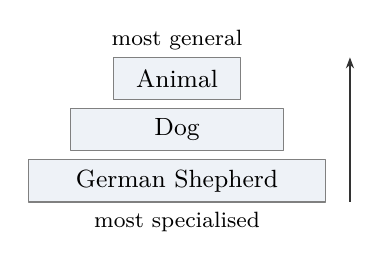
\begin{tikzpicture}[line join=round]
\node[,inner sep=1pt,font=\footnotesize] at (2.340,-0.216) {most general};
\filldraw[draw=black!50,fill=Paperblue] (1.530,-0.432) rectangle (3.150,-0.972);
\node[,inner sep=1pt,font=\small] at (2.340,-0.702) {Animal};
\filldraw[draw=black!50,fill=Paperblue] (0.990,-1.080) rectangle (3.690,-1.620);
\node[,inner sep=1pt,font=\small] at (2.340,-1.350) {Dog};
\filldraw[draw=black!50,fill=Paperblue] (0.450,-1.728) rectangle (4.230,-2.268);
\node[,inner sep=1pt,font=\small] at (2.340,-1.998) {German Shepherd};
\draw[-{Stealth[length=4pt]},black!80] (4.536,-2.268) -- (4.536,-0.432);
\node[,inner sep=1pt,font=\footnotesize] at (2.340,-2.520) {most specialised};
\end{tikzpicture}\par\smallskip{\small\raggedright \textbf{One branch of the animal hierarchy.} The German Shepherd inherits from Dog, which inherits from Animal.\par}\end{minipage}
\end{center}

\Needspace{6\baselineskip}
Cat, Rabbit, and Dog can each extend Animal. A Cat may add \texttt{speak()}; a plain Animal does not gain that Cat-only method. When a Dog inherits \texttt{get\_age()}, Python finds it in Animal if Dog does not define its own version.

\Needspace{5\baselineskip}
\Needspace{6\baselineskip}
\begin{notebox}\textbf{Trap:} Inheriting a method does not copy its definition into the subclass’s source; lookup finds it through the hierarchy.\end{notebox}

\Needspace{10\baselineskip}
\begin{notebox}\textbf{Near miss:} Calling \texttt{animal.speak()} is not valid merely because Cat defines \texttt{speak}; the object’s class must provide that method.\end{notebox}

\begin{recallbox}{Recall \ensuremath{\cdot} §11.4}
\Needspace{4\baselineskip}
\begin{enumerate}
\item Where does lookup start?
\item Does an Animal instance acquire Cat-only methods?
\end{enumerate}

\nopagebreak[4]{\small\itshape Answers: see “11.4 Inheritance and method lookup” under Answers at the end.}
\end{recallbox}
\end{keepsection}

\begin{keepsection}
\Needspace{12\baselineskip}
\section{11.5 Extending and overriding}

\Needspace{9\baselineskip}
\begin{plainbox}\textbf{In plain words:} a subclass can add state, extend behaviour, or \textbf{override} a method with its own version.\end{plainbox}

\begin{equationcard}{Override selection}
\[ \begin{gathered} \texttt{same method name in subclass \ensuremath{\to} subclass version runs} \end{gathered} \]
{\small \emph{Read it as: “the closest matching definition wins”.}\par If it is absent, lookup continues upward.}
\end{equationcard}

\Needspace{12\baselineskip}
Dog can initialise its own name and age by calling \texttt{Animal.\_\_init\_\_(self, age)}, then add a friends list. It can add \texttt{add\_friend} and \texttt{age\_diff}, and override \texttt{\_\_str\_\_} to print a dog-specific prefix. Shepherd can inherit from Dog, call Dog’s initialiser, add a skill, and override \texttt{speak} and \texttt{\_\_str\_\_}. In a single-inheritance chain, the first definition found supplies the behaviour.

\begin{workedbox}{Worked example \ensuremath{\cdot} Dog initialisation}
\Needspace{7\baselineskip}
\begin{enumerate}
\item Call \texttt{Dog("Rex", 4)}.
\item Dog passes age 4 to the Animal initialiser, which stores age and initialises name.
\item Dog sets the supplied name through \texttt{set\_name} and creates its own friends list.
\item A Dog’s \texttt{\_\_str\_\_} is found before Animal’s; inherited getters still resolve to Animal.
\end{enumerate}
\end{workedbox}

\Needspace{6\baselineskip}
This lecture uses an explicit parent call. Python also provides \texttt{super()}, which follows the method resolution order and is less tied to a named parent class; that is a modern extension to the lecture’s example.

\Needspace{5\baselineskip}
\Needspace{6\baselineskip}
\begin{notebox}\textbf{Trap:} If a subclass defines \texttt{\_\_init\_\_}, it must call the parent initialiser itself when parent state is still needed.\end{notebox}

\Needspace{10\baselineskip}
\begin{notebox}\textbf{Near miss:} Defining Dog’s \texttt{\_\_str\_\_} replaces the Animal version for Dogs; it does not automatically append the parent’s text.\end{notebox}

\begin{recallbox}{Recall \ensuremath{\cdot} §11.5}
\Needspace{4\baselineskip}
\begin{enumerate}
\item What should Dog do before adding its own state?
\item Which string method runs for a Shepherd?
\end{enumerate}

\nopagebreak[4]{\small\itshape Answers: see “11.5 Extending and overriding” under Answers at the end.}
\end{recallbox}
\end{keepsection}

\begin{keepsection}
\Needspace{11\baselineskip}
\section{11.6 Class variables and IDs}

\Needspace{8\baselineskip}
\begin{plainbox}\textbf{In plain words:} a \textbf{class variable} is shared by instances that use the class.\end{plainbox}

\begin{equationcard}{Rabbit ID assignment}
\[ \begin{gathered} \texttt{self.rid = Rabbit.tag; Rabbit.tag = Rabbit.tag + 1} \end{gathered} \]
{\small \emph{Read it as: “copy the shared next number to this rabbit, then advance the shared counter”.}\par Initialise \texttt{Rabbit.tag} once in the class.}
\end{equationcard}

\Needspace{11\baselineskip}
Rabbit can start with class variable \texttt{tag = 1}. Each new instance stores the current tag in its own \texttt{rid}, then increments \texttt{Rabbit.tag}. The next instance receives the next number. A getter can format the ID with leading zeros, such as \texttt{001}.

\begin{workedbox}{Worked example \ensuremath{\cdot} unique IDs}
\Needspace{7\baselineskip}
\begin{enumerate}
\item Initially \texttt{Rabbit.tag} is 1.
\item The first Rabbit stores \texttt{rid = 1}, then the class counter becomes 2.
\item The next stores \texttt{rid = 2}, then the counter becomes 3.
\item The earlier instance keeps its own \texttt{rid} while the shared counter advances.
\end{enumerate}
\end{workedbox}

\Needspace{5\baselineskip}
\Needspace{6\baselineskip}
\begin{notebox}\textbf{Trap:} Store each ID on the instance; do not use the changing class counter as though it were that rabbit’s ID.\end{notebox}

\Needspace{10\baselineskip}
\begin{notebox}\textbf{Near miss:} Incrementing \texttt{self.tag} can create an instance attribute and leave the shared class counter unchanged; update \texttt{Rabbit.tag}.\end{notebox}

\begin{recallbox}{Recall \ensuremath{\cdot} §11.6}
\Needspace{4\baselineskip}
\begin{enumerate}
\item Which value is shared, and which belongs to one Rabbit?
\item Why save an instance ID before incrementing the counter?
\end{enumerate}

\nopagebreak[4]{\small\itshape Answers: see “11.6 Class variables and IDs” under Answers at the end.}
\end{recallbox}
\end{keepsection}

\begin{keepsection}
\Needspace{12\baselineskip}
\section{11.7 Operators and Rabbit equality}

\Needspace{9\baselineskip}
\begin{plainbox}\textbf{In plain words:} special methods let a class give familiar syntax a meaning that fits its objects.\end{plainbox}

\begin{equationcard}{Rabbit operations}
\[ \begin{gathered} \texttt{r1 + r2 \ensuremath{\to} \_\_add\_\_; r1 == r2 \ensuremath{\to} \_\_eq\_\_} \end{gathered} \]
{\small \emph{Read it as: “addition calls \_\_add\_\_; equality calls \_\_eq\_\_”.}\par Choose an explicit rule for each operation.}
\end{equationcard}

\Needspace{11\baselineskip}
Rabbit addition can create a new Rabbit of age 0 whose parents are the two operands. Equality can mean “the same two parents”, regardless of parent order. Compare unique parent IDs rather than invoking Rabbit equality recursively on the parent objects.

\begin{workedbox}{Worked example \ensuremath{\cdot} unordered parent pair}
\Needspace{7\baselineskip}
\begin{enumerate}
\item Rabbit A has parents with IDs 4 and 9; Rabbit B has the same IDs in reverse order.
\item The ordered test fails because 4 \ensuremath{\neq} 9 in the first position.
\item The reversed test succeeds: A’s first parent matches B’s second, and vice versa.
\item The rabbits compare equal under the stated parent-pair rule.
\end{enumerate}
\end{workedbox}

\Needspace{6\baselineskip}
There is an edge case in the lecture’s example: parent fields default to \texttt{None}. A safe equality method must handle \texttt{None} before reading \texttt{.rid}; otherwise comparing root rabbits raises \texttt{AttributeError}. Define whether two absent parents count as matching, then compare real parents by ID.

\Needspace{5\baselineskip}
\Needspace{6\baselineskip}
\begin{notebox}\textbf{Trap:} An equality method that calls \texttt{self.parent1 == other.parent1} may invoke Rabbit’s equality again and recurse down the family tree.\end{notebox}

\Needspace{10\baselineskip}
\begin{notebox}\textbf{Near miss:} Comparing only corresponding parent positions says reversed parent order is unequal; also check the swapped pairing.\end{notebox}

\begin{recallbox}{Recall \ensuremath{\cdot} §11.7}
\Needspace{4\baselineskip}
\begin{enumerate}
\item What does Rabbit addition return in the lecture design?
\item How does the equality rule treat parent order?
\end{enumerate}

\nopagebreak[4]{\small\itshape Answers: see “11.7 Operators and Rabbit equality” under Answers at the end.}
\end{recallbox}
\end{keepsection}

\begin{keepsection}
\Needspace{4\baselineskip}
\section{Decision map}
\end{keepsection}

\begin{keepsection}
\Needspace{11\baselineskip}
\section{Derive it cold}

\Needspace{8\baselineskip}
\begin{enumerate}
\item Trace \texttt{get\_age()} after the internal field changes from age to years. \hfill{\small\color{FAUblue}§11.2}
\item Follow method lookup for Shepherd \ensuremath{\to} Dog \ensuremath{\to} Animal. \hfill{\small\color{FAUblue}§11.4}
\item Trace Dog’s parent and child initialisation. \hfill{\small\color{FAUblue}§11.5}
\item Generate the first three Rabbit IDs from \texttt{tag = 1}. \hfill{\small\color{FAUblue}§11.6}
\item Derive Rabbit equality for equal, reversed, and missing parents. \hfill{\small\color{FAUblue}§11.7}
\end{enumerate}
\end{keepsection}

\begin{keepsection}
\Needspace{14\baselineskip}
\section{Explain it}

\Needspace{11\baselineskip}
\begin{enumerate}
\item Why keep the getter name stable when representation changes?
\item Why is Python’s getter/setter style not strict privacy?
\item When does a default argument apply?
\item Why does a subclass inherit a constructor if it defines none?
\item Why does an override in Shepherd win over Dog’s version?
\item Why store an ID on each Rabbit?
\item Why compare parent IDs instead of parent objects?
\end{enumerate}

\nopagebreak[4]{\small\itshape Answers: see “Explain it” under Answers at the end.}
\end{keepsection}

\clearpage

\begin{keepsection}
\Needspace{9\baselineskip}
\section{Mixed practice}

\Needspace{6\baselineskip}
20 problems. Try each before opening its worked answer.

\begin{enumerate}
\item What are data attributes and methods intended to describe?
\item Why prefer \texttt{a.get\_age()} to \texttt{a.age}?
\item With \texttt{set\_name(self, newname="")}, what does \texttt{a.set\_name()} store?
\item Where does method lookup begin for a Shepherd instance?
\item What should Dog call before setting its own name and friends list?
\item Which object shares \texttt{Rabbit.tag}?
\item Which method defines \texttt{r1 + r2}?
\item If Dog has no \texttt{get\_age}, where is it found?
\item Which \texttt{\_\_str\_\_} runs on a Shepherd if Shepherd overrides it?
\item Which method defines \texttt{r1 == r2}?
\item How can Animal rename its field without changing callers?
\item Tags start at 1. Which IDs do the first three rabbits receive?
\item What can go wrong comparing two root rabbits by parent \texttt{.rid}?
\item What happens if a caller passes \texttt{"Fluffy"} to \texttt{set\_name}?
\item Can an Animal instance call Cat’s new \texttt{speak} method?
\item Why call the parent constructor in Dog?
\item After the first rabbit stores ID 1, what is the next class tag?
\item How should equality handle parents in reversed order?
\item Do getters prevent external writes to \texttt{a.age}?
\item Why group related methods in a class?
\end{enumerate}

\nopagebreak[4]{\small\itshape Answers: see “Mixed practice” under Answers at the end.}
\end{keepsection}

\begin{keepsection}
\Needspace{5\baselineskip}
\section{Exam-style problems}

Allow about 20 minutes per problem.

\begin{keepsection}
\Needspace{13\baselineskip}
\subsection{Problem 1 \ensuremath{\cdot} Animal hierarchy}

\Needspace{10\baselineskip}
Animal defines age accessors and \texttt{\_\_str\_\_}. Dog inherits Animal, initialises a friends list, and overrides \texttt{\_\_str\_\_}. Shepherd inherits Dog, adds skill, and overrides \texttt{speak}.

\Needspace{7\baselineskip}
\begin{enumerate}
\item Trace which initialisers run when creating a Shepherd.
\item Give the method lookup order for \texttt{get\_age} and \texttt{\_\_str\_\_}.
\item Can an Animal object call Shepherd’s \texttt{speak}? Explain.
\item Why use \texttt{get\_age()} when Animal renames its field?
\end{enumerate}

\nopagebreak[4]{\small\itshape Answers: see “Exam-style problems” under Answers at the end.}
\end{keepsection}

\begin{keepsection}
\Needspace{13\baselineskip}
\subsection{Problem 2 \ensuremath{\cdot} Rabbit family operators}

\Needspace{10\baselineskip}
Rabbit stores a class counter, an instance ID, and two optional parent references. Define what addition and equality should mean, including edge cases.

\Needspace{7\baselineskip}
\begin{enumerate}
\item Trace IDs for three newly constructed Rabbits when the tag starts at 1.
\item Describe the result of \texttt{r1 + r2}.
\item State a symmetric same-parent equality rule.
\item Handle root rabbits whose parent fields are \texttt{None}.
\end{enumerate}

\nopagebreak[4]{\small\itshape Answers: see “Exam-style problems” under Answers at the end.}
\end{keepsection}
\end{keepsection}

\begin{keepsection}
\Needspace{16\baselineskip}
\section{Slips in the notes}

\Needspace{13\baselineskip}
\begin{itemize}
\item Slides 6–7, 13 and 19 show malformed constructor spellings or calls (for example, \texttt{def\_init\_} and \texttt{Animal.\_init\_}). Valid Python uses \texttt{def \_\_init\_\_} and \texttt{Animal.\_\_init\_\_}.
\item Slides 7, 13, 14 and 17 miss or misplace underscores around the string hook (for example, \texttt{def\_str\_\_} or \texttt{def str}). The special method is \texttt{def \_\_str\_\_(self):}.
\item Slide 21’s code label is rendered as \texttt{def\_eq\_}, which is not a Python method definition. The intended special method is \texttt{def \_\_eq\_\_(self, other):}; the slide’s accompanying text refers to \texttt{\_\_eq\_\_}.
\item The Rabbit equality example dereferences each parent’s \texttt{rid}, although both parent parameters default to \texttt{None}. Comparing root rabbits would therefore raise \texttt{AttributeError}. This guide calls out the required missing-parent case.
\end{itemize}
\end{keepsection}

\begin{keepsection}
\Needspace{7\baselineskip}
\section{Self-check}

\begin{enumerate}
\item $\mdlgwhtsquare$\  I separate class, instance, data and behaviour (1, 20).
\item $\mdlgwhtsquare$\  I explain getters and Python’s information-hiding limit (2, 11, 19).
\item $\mdlgwhtsquare$\  I trace default and supplied arguments (3, 14).
\item $\mdlgwhtsquare$\  I trace inheritance and method lookup (4, 8, 15).
\item $\mdlgwhtsquare$\  I trace an overridden method (9).
\item $\mdlgwhtsquare$\  I trace parent initialisation (5, 16).
\item $\mdlgwhtsquare$\  I distinguish subclass-only and inherited methods (8, 15).
\item $\mdlgwhtsquare$\  I derive shared counters and instance IDs (6, 12, 17).
\item $\mdlgwhtsquare$\  I map operators to special methods (7, 10).
\item $\mdlgwhtsquare$\  I reason about Rabbit equality and missing parents (13, 18).
\item $\mdlgwhtsquare$\  I rebuild the five derivations.
\item $\mdlgwhtsquare$\  I solve both exam problems.
\end{enumerate}
\end{keepsection}


\clearpage
\section{Answers}
\begin{keepsection}\subsection{Start from memory}

\Needspace{9\baselineskip}
\begin{enumerate}
\item The class can change its internal attribute name without changing callers. \hfill{\small\color{FAUblue}§11.2}
\item In the current class first, then upward through its superclass chain. \hfill{\small\color{FAUblue}§11.4}
\item Call the parent initialiser, then assign the subclass’s own attributes. \hfill{\small\color{FAUblue}§11.5}
\item Read the shared counter, store that value on the instance, then increment the class counter. \hfill{\small\color{FAUblue}§11.6}
\item Rabbit equality may compare the parents again until it reaches \texttt{None}. \hfill{\small\color{FAUblue}§11.7}
\end{enumerate}

\end{keepsection}
\begin{keepsection}\subsection{11.1 Classes and object roles}

\Needspace{4\baselineskip}
\begin{enumerate}
\item The representation and the methods that define how the object is used. \hfill{\small\color{FAUblue}§11.1}
\item Their instance-attribute values; their class is shared. \hfill{\small\color{FAUblue}§11.1}
\end{enumerate}

\end{keepsection}
\begin{keepsection}\subsection{11.2 Getters and information hiding}

\Needspace{4\baselineskip}
\begin{enumerate}
\item Keep its public method name and update its implementation to read the new field. \hfill{\small\color{FAUblue}§11.2}
\item No. They provide a stable interface by convention; direct access remains possible. \hfill{\small\color{FAUblue}§11.2}
\end{enumerate}

\end{keepsection}
\begin{keepsection}\subsection{11.3 Defaults and Animal methods}

\Needspace{4\baselineskip}
\begin{enumerate}
\item The empty string. \hfill{\small\color{FAUblue}§11.3}
\item Pass it, for example \texttt{set\_name("Fluffy")}. \hfill{\small\color{FAUblue}§11.3}
\end{enumerate}

\end{keepsection}
\begin{keepsection}\subsection{11.4 Inheritance and method lookup}

\Needspace{4\baselineskip}
\begin{enumerate}
\item In the instance’s class, then its superclass chain. \hfill{\small\color{FAUblue}§11.4}
\item No; Cat’s added behaviour belongs to Cat instances and its subclasses. \hfill{\small\color{FAUblue}§11.4}
\end{enumerate}

\end{keepsection}
\begin{keepsection}\subsection{11.5 Extending and overriding}

\Needspace{4\baselineskip}
\begin{enumerate}
\item Call the parent initialiser to establish inherited state. \hfill{\small\color{FAUblue}§11.5}
\item The nearest definition: Shepherd’s if present, otherwise Dog’s, then Animal’s. \hfill{\small\color{FAUblue}§11.5}
\end{enumerate}

\end{keepsection}
\begin{keepsection}\subsection{11.6 Class variables and IDs}

\Needspace{4\baselineskip}
\begin{enumerate}
\item \texttt{Rabbit.tag} is shared; \texttt{self.rid} belongs to one object. \hfill{\small\color{FAUblue}§11.6}
\item So the instance keeps its assigned unique number as the shared counter moves on. \hfill{\small\color{FAUblue}§11.6}
\end{enumerate}

\end{keepsection}
\begin{keepsection}\subsection{11.7 Operators and Rabbit equality}

\Needspace{4\baselineskip}
\begin{enumerate}
\item A new age-0 Rabbit whose parent fields reference the two operands. \hfill{\small\color{FAUblue}§11.7}
\item It accepts either the same order or the reversed order. \hfill{\small\color{FAUblue}§11.7}
\end{enumerate}

\end{keepsection}
\begin{keepsection}\subsection{Explain it}

\Needspace{11\baselineskip}
\begin{enumerate}
\item Callers depend on a stable interface, not the internal field name. \hfill{\small\color{FAUblue}§11.2}
\item Callers can still directly read, change, or add attributes. \hfill{\small\color{FAUblue}§11.2}
\item When that argument is omitted from the call. \hfill{\small\color{FAUblue}§11.3}
\item Lookup proceeds to the superclass when the subclass has no method with that name. \hfill{\small\color{FAUblue}§11.4}
\item Lookup starts in Shepherd and stops at the first matching definition. \hfill{\small\color{FAUblue}§11.4}
\item The class counter changes; the instance needs to keep its assigned number. \hfill{\small\color{FAUblue}§11.6}
\item Direct equality may recursively invoke Rabbit’s method and fail at a missing parent. \hfill{\small\color{FAUblue}§11.7}
\end{enumerate}

\end{keepsection}
\begin{keepsection}\subsection{Mixed practice}

\begin{enumerate}
\item Attributes describe what an object is; methods describe what it does. \hfill{\small\color{FAUblue}§11.1}
\item The class can change its representation while keeping callers stable. \hfill{\small\color{FAUblue}§11.2}
\item The empty string. \hfill{\small\color{FAUblue}§11.3}
\item In Shepherd, then Dog, then Animal. \hfill{\small\color{FAUblue}§11.4}
\item Call \texttt{Animal.\_\_init\_\_(self, age)} to initialise inherited state. \hfill{\small\color{FAUblue}§11.5}
\item The Rabbit class and its instances. \hfill{\small\color{FAUblue}§11.6}
\item \texttt{\_\_add\_\_}. \hfill{\small\color{FAUblue}§11.7}
\item In Animal, where the inherited method is defined. \hfill{\small\color{FAUblue}§11.4}
\item Shepherd’s override. \hfill{\small\color{FAUblue}§11.5}
\item \texttt{\_\_eq\_\_}. \hfill{\small\color{FAUblue}§11.7}
\item Keep \texttt{get\_age()} as the public interface and change its body to read the renamed field. \hfill{\small\color{FAUblue}§11.2}
\item 1, 2, and 3; the shared tag increments after each assignment. \hfill{\small\color{FAUblue}§11.6}
\item \texttt{None.rid} raises AttributeError; handle missing parents before reading IDs. \hfill{\small\color{FAUblue}§11.7}
\item The supplied name is stored instead of the default. \hfill{\small\color{FAUblue}§11.3}
\item No. That method belongs to Cat and subclasses of Cat. \hfill{\small\color{FAUblue}§11.4}
\item So Animal’s age and name state is initialised. \hfill{\small\color{FAUblue}§11.5}
\item 2. \hfill{\small\color{FAUblue}§11.6}
\item Check both the same-order pairing and the swapped pairing. \hfill{\small\color{FAUblue}§11.7}
\item No; direct attribute access remains possible in Python. \hfill{\small\color{FAUblue}§11.2}
\item They keep related behaviour together, aiding modularity and reuse. \hfill{\small\color{FAUblue}§11.1}
\end{enumerate}

\end{keepsection}
\begin{keepsection}\subsection{Exam-style problems}

\Needspace{10\baselineskip}
\begin{enumerate}
\item Shepherd initialisation calls Dog’s initialiser, which calls Animal’s; each then stores its own fields. \hfill{\small\color{FAUblue}§11.5}
\item \texttt{get\_age} is found in Animal. \texttt{\_\_str\_\_} is found in Shepherd if overridden there, otherwise Dog, then Animal. \hfill{\small\color{FAUblue}§11.4, §11.5}
\item No. Lookup on an Animal instance searches Animal and its ancestors; it does not search subclasses. \hfill{\small\color{FAUblue}§11.4}
\item The getter keeps callers independent of the internal field name. \hfill{\small\color{FAUblue}§11.2}
\end{enumerate}

\end{keepsection}
\begin{keepsection}\subsection{Exam-style problems}

\Needspace{8\baselineskip}
\begin{enumerate}
\item They receive IDs 1, 2, and 3; the shared counter advances after each. \hfill{\small\color{FAUblue}§11.6}
\item \texttt{\_\_add\_\_} returns a new age-0 Rabbit with r1 and r2 as its parents. \hfill{\small\color{FAUblue}§11.7}
\item Match both IDs in the same order or both in the reversed order. \hfill{\small\color{FAUblue}§11.7}
\item Compare absent values explicitly (for example, None with None) before reading IDs; compare two real parent objects by their unique IDs. \hfill{\small\color{FAUblue}§11.7}
\end{enumerate}

\end{keepsection}

\vfill{\small Based on the supplied “11\_Classes and Inheritance.pdf”, rewritten in my own words. Python inheritance and method lookup follow the Python classes tutorial; special method names follow the data model. \texttt{super()} follows the built-in reference. Not an official FAU publication; check course details against current notes. Made by \textbf{Thanate Amornjiraporn (Focus)}.}

\end{document}
